\documentclass[a4paper,12pt]{UoBnote}

\usepackage{enumitem}
\usepackage{listings}
\usepackage{color}
\usepackage{graphicx}
\usepackage{amsfonts}
\usepackage[backend=bibtex]{biblatex}

\addbibresource{bilbo.bib}

\lstset{language=sh}
\setlength{\parskip}{1em}
\author{Mike Knee}

\shorttitle{Numerical Modelling}
\title{Worksheet 2 Report}
\date{\today}
\issue{1}

\begin{document}

\maketitle
\tableofcontents
\vspace{1cm}\hrule \vspace{1cm}

\section{Question 2}

Here we are using two numerical methods, the trapezium method and then Simpson's rule to evaluate the integral
\[\int_{0}^{2} e^{-x}\sin{x} dx\]
As we can evaluate this integral analytically we will do that first in order to have some refernce value which we can compare our results to. We use integration by parts to solve this integral
\[I = \int_{0}^{2} e^{-x}\sin{x} dx \]
\[I = \left[ -e^{-x}\cos{x} \right]_{0}^{2} + \int_{0}^{2} e^{-x}\cos{x} dx \]
and then applying integration by parts again
\[I = \left[ -e^{-x}\cos{x} \right]_{0}^{2} + \left[ -e^{-x}\sin{x} \right]_{0}^{2} - \int_{0}^{2} e^{-x}\sin{x} dx \] 
\[I = \left[ -e^{-x}\cos{x} \right]_{0}^{2} + \left[ -e^{-x}\sin{x} \right]_{0}^{2} - I \] 
\[2I = \left[ -e^{-x}\cos{x} \right]_{0}^{2} + \left[ -e^{-x}\sin{x} \right]_{0}^{2} \] 
\[2I = 1 - e^{-2}(\cos{2}+\sin{2}) \]
And now all that's left to do is ask a calculator to provide us with the answer.

\begin{figure}
	\centering
	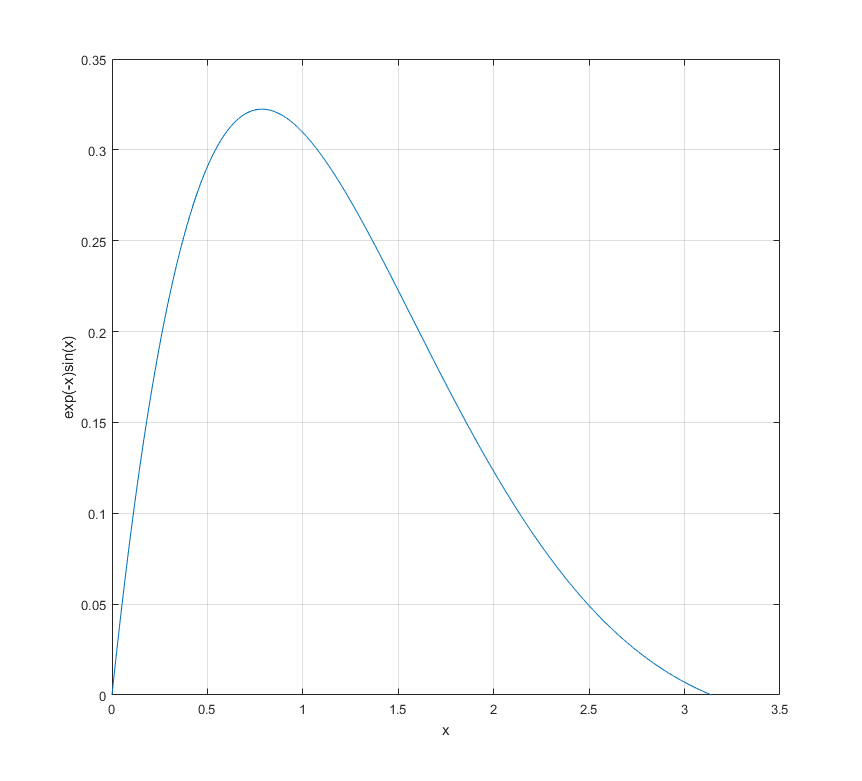
\includegraphics[scale=0.7]{ExpSin}
	\caption{Plot of $f(x)=e^{-x}\sin{x}$}
	\label{fig:expsin}
\end{figure}

Figure \ref{fig:expsin} shows a plot of $e^{-x}\sin{x}$ against $x$. The source file for a program that caluclates the area under this curve using both the trapezium and Simpson's rule is called ``question2.cpp''.

\printbibliography

\end{document}

